\documentclass[c]{beamer}
\usetheme{default}
\title{Generalizing Nondeterminism for Algebraic Computation Machines}
\author{Scott Sanderson}
\institute{Department of Mathematics\\Williams College}
\date{\today}
\usepackage{tikz}
\usepackage{beamerthesiscommands}
\usepackage{mydiagrams}
\usepackage{graphicx}
\usepackage{algorithm}
\usepackage{algorithmicx}
\usepackage{algpseudocode}
\usepackage{url}
\renewcommand{\algorithmicrequire}{\textbf{Input:}}
% \usepackage{enumitem}
\usetikzlibrary{calc,arrows,shapes,positioning}

\begin{document}

\theoremstyle{definition}
\newtheorem{proposition}{Proposition}
\newtheorem{proofidea}{Proof Idea}

\begin{frame}
  \titlepage
\end{frame}

\begin{frame}{Computability and Complexity Theory}
  
  \begin{columns}
    \visible<1->{
      \column{0.5\textwidth}
      \begin{figure}[h]
        \centering \scaletopagewidth{\algoyesno{}}
      \end{figure}
    }
    \visible<2->{
      \column{0.6\textwidth}
      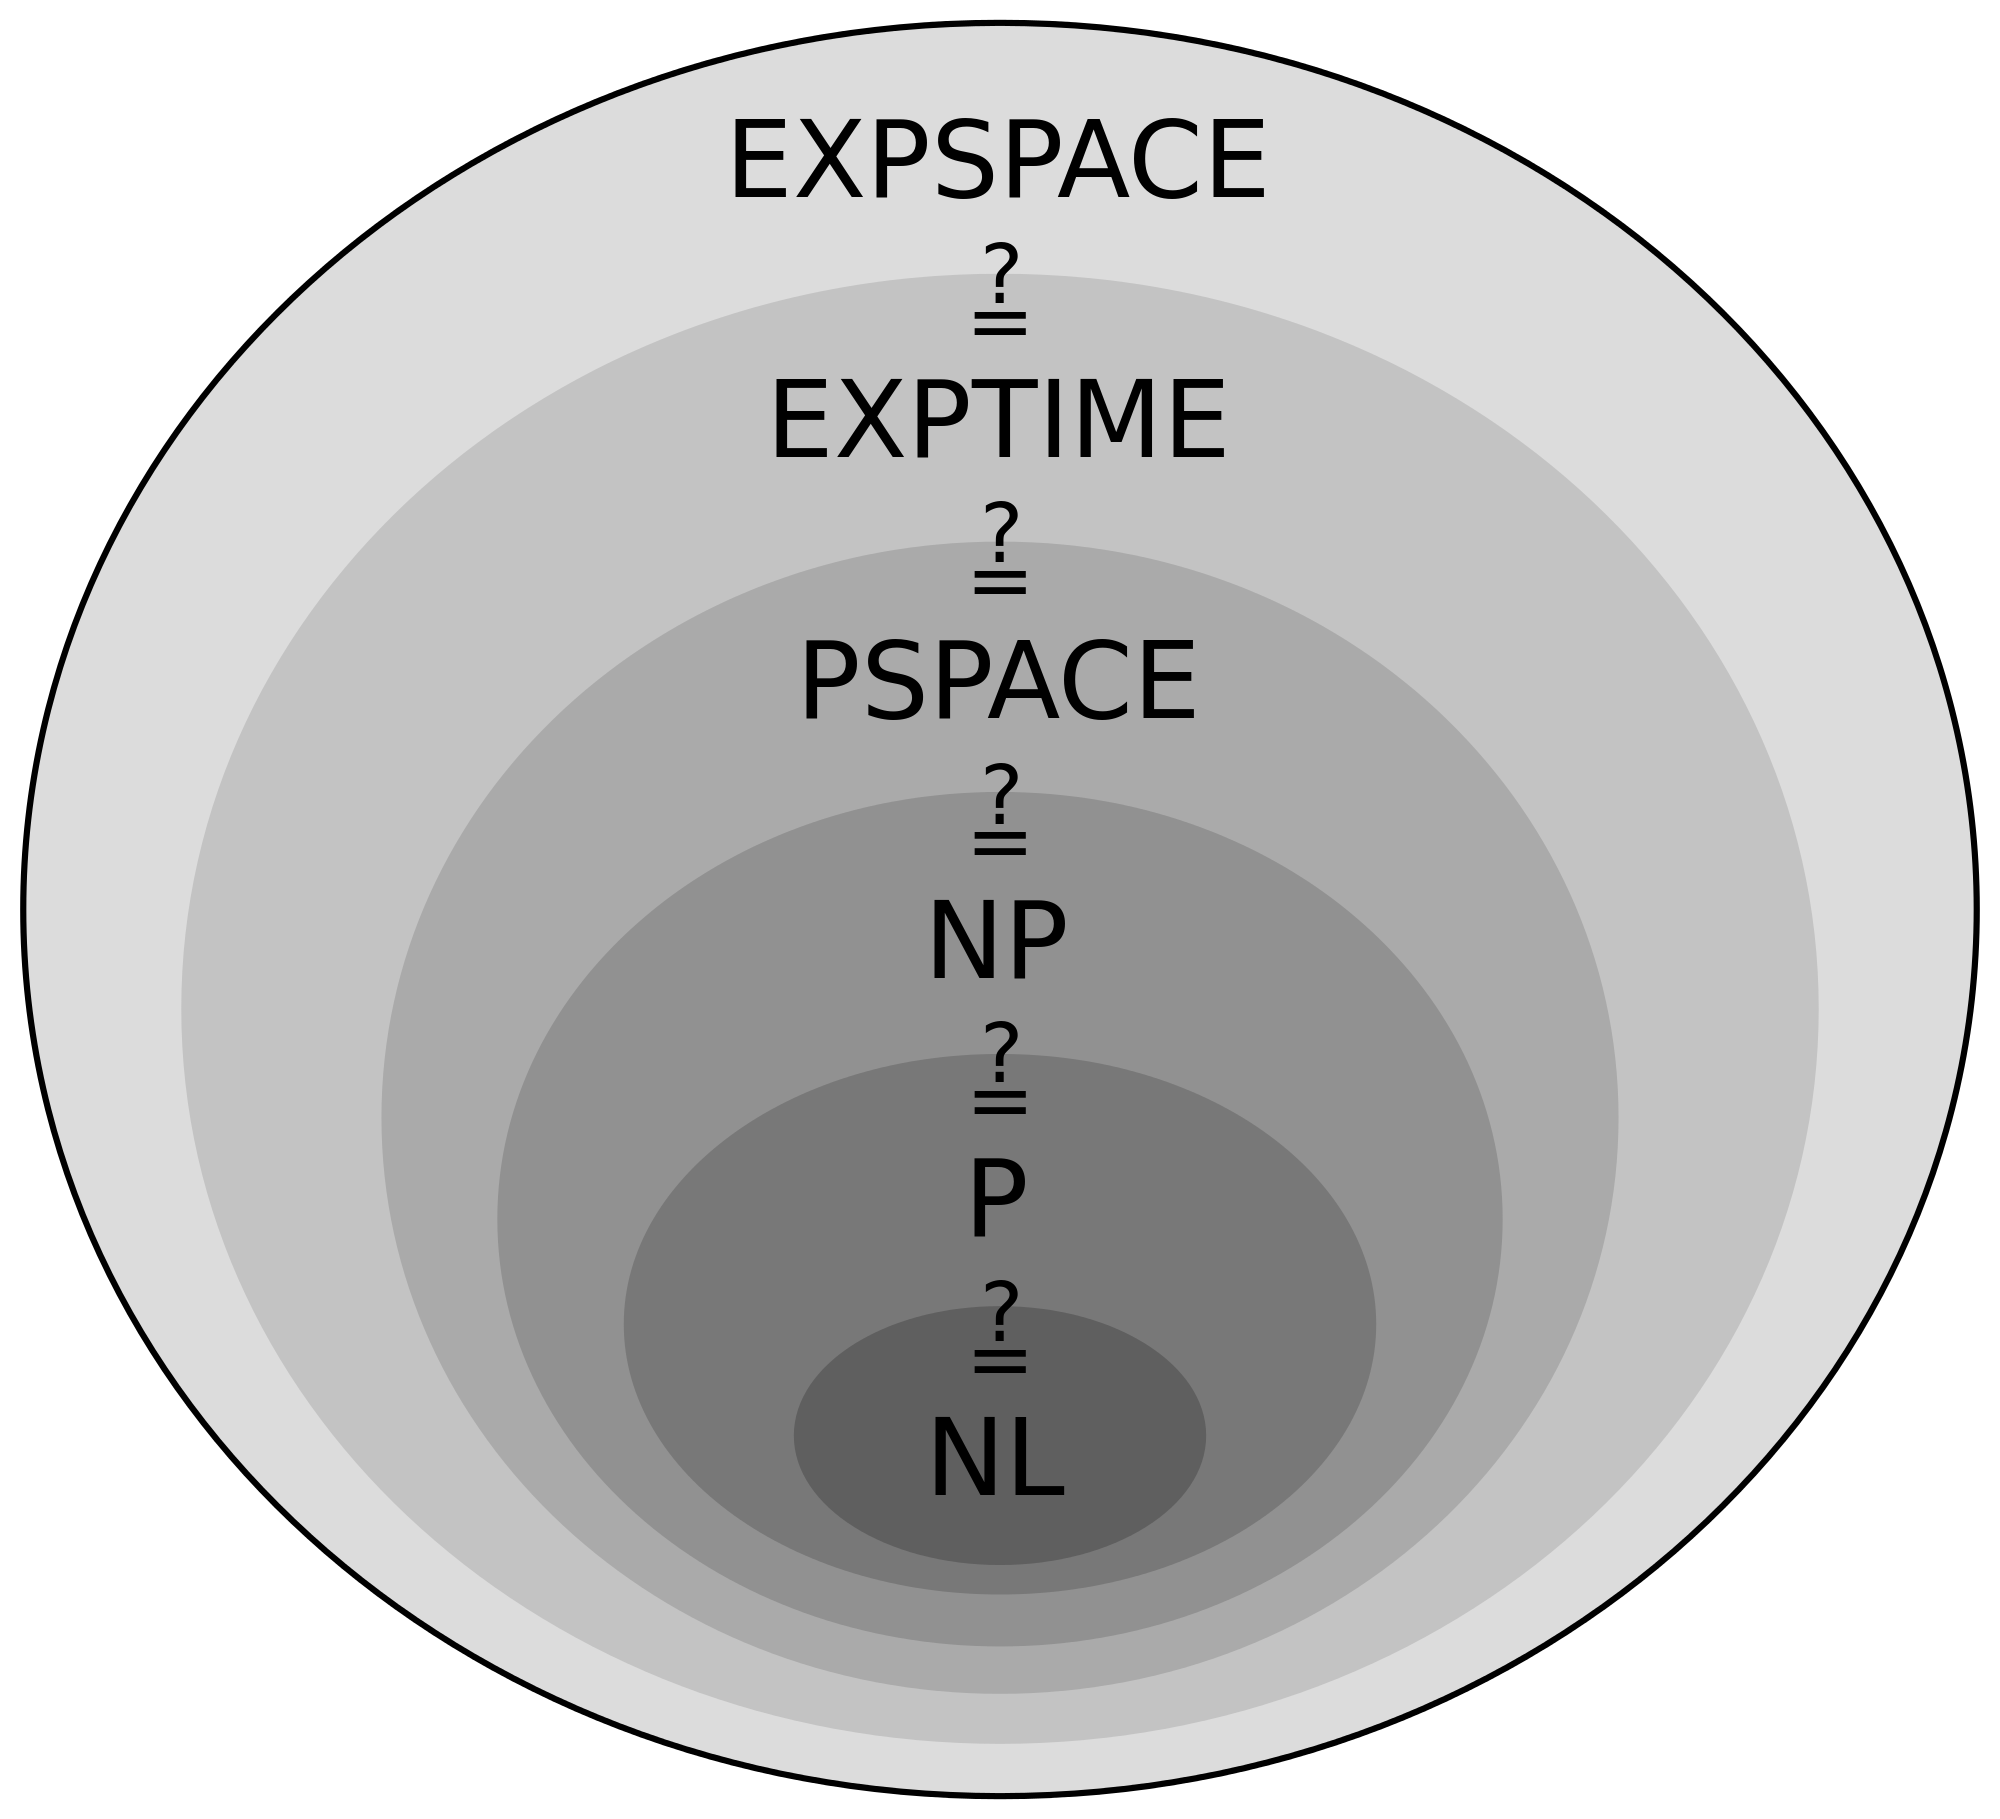
\includegraphics[width=\textwidth]{media/complexity.png}    
    }
  \end{columns}

\end{frame}

\begin{frame}{Outline}
  \begin{center}
    \scaletopagewidth{\outlinenobss}
  \end{center}
\end{frame}

\begin{frame}{Outline}
  \begin{center}
    \scaletopagewidth{\outlinenondet}
  \end{center}
\end{frame}

\begin{frame}{Outline}
  \begin{center}
    \scaletopagewidth{\outlinealmostfinal}
  \end{center}
\end{frame}

\begin{frame}{Outline}
  \begin{center}
    \scaletopagewidth{\outlinefinal}
  \end{center}
\end{frame}

\begin{frame}{A Simple Puzzle}
  
  \begin{itemize}
    \setlength{\itemsep}{4mm}
  \item[] Does the set: $\set{1,4,7,-5,-3,18,-6,12}$ contain
    a subset adding up to 10? \pause
  \item[] Yes.  \textbf{Proof}: $18 - 3 - 6 + 1 = 10$ \pause
  \item[] Does $\set{1, 17, 25, -3, 11, -9, 22, 13}$ contain a subset
    adding up to 7?\pause
  \item[] No.  \textbf{Proof}: ...try them all? 
  \end{itemize}
  
\end{frame}

\begin{frame}{\subsum{}}

  An \textbf{instance} of \subsum{} is a pair $(S, t)$, where:

    \begin{itemize}
    \item $S = \set{s_1, s_2, \ldots, s_n}$ is a set of integers.
    \item $t$ is a single integer, called the \textbf{target} for $S$.
    \end{itemize}\pause

    \vspace{\baselineskip}

    An instance of \subsum{} is a \textbf{Yes Instance} if
    there exists some $X \subseteq S$ such that $\sum_X = t$.

    \vspace{\baselineskip}
    
    Otherwise it is a \textbf{No Instance}.
\end{frame}

\begin{frame}{Decision Problems}

  \begin{itemize}
  \item[] \subsum{} is an example of a \textbf{Decision Problem}.\pause

    \vspace{\baselineskip}

  \item[] A Decision Problem $D$ is a set of values, partitioned into
    Yes Instances and No Instances, $D_{yes}$ and $D_{no}$.

    \vspace{\baselineskip}

  \item[] Goal: find an algorithm that ``accepts'' $D_{yes}$ and
    ``rejects'' $D_{no}$.  Such an algorithm \textbf{decides} $D$.
  \end{itemize}

\end{frame}

\begin{frame}{Classical Machine Model - Turing Machines}
  \begin{columns}

    \column{0.5\textwidth}
    \begin{itemize}
    \item[] Infinite one-way tape, divided into cells.    
    \end{itemize}
    \column{0.5\textwidth}
    \scaletopagewidth{\tape{$q$}{{1,0,1,0,0,$\blank$, $\blank$, $\cdots$}}}
  \end{columns}
\end{frame}

\begin{frame}{Classical Machine Model - Turing Machines}
  \begin{columns}

    \column{0.5\textwidth}
    \begin{itemize}
    \item At each step, tape head reads a symbol, writes a symbol,
      moves left/right, and changes state.
    \end{itemize}
    
    \column{0.5\textwidth}
    \scaletopagewidth{\tape[1]{$q$}{{1,0,1,0,0,$\blank$, $\blank$, $\cdots$}}}
    $$\delta(q, 1) = (q', 0, \rightarrow)$$
    \scaletopagewidth{\tape[2]{$q'$}{{0,0,1,0,0,$\blank$, $\blank$, $\cdots$}}}
  \end{columns}
\end{frame}

\begin{frame}{Turing Machines}
  \begin{columns}

    \column{0.5\textwidth}
    \begin{itemize}
    \item Computation ends when we enter special states $q_{accept}$
      or $q_{reject}$.
    \end{itemize}
    \column{0.5\textwidth}
    \scaletopagewidth{\tape[3]{$q'$}{{0,1,1,0,0,$\blank$, $\blank$, $\cdots$}}}
    $$\delta(q', 1) = (q_{acc}, 1, \leftarrow)$$
    \scaletopagewidth{\tape[2]{$q_{acc}$}{{0,1,1,0,0,$\blank$, $\blank$, $\cdots$}}}
  \end{columns}
\end{frame}

\begin{frame}{Turing Machine Example - Even or Odd?}
  \begin{columns}[c]
    
    \small

    \column{0.5\textwidth}

    \begin{itemize}
    \item[] $Q = \set{q_0, q_1, q_{acc}, q_{rej}}$
    \item[] $\Gamma = \set{\blank, 0, 1}$
    \item[] $\Sigma = \set{0,1}$
    \item[] $\delta(q_0, 0) = (q_0, \blank, \rightarrow)$
    \item[] $\delta(q_0, 1) = (q_1, \blank, \rightarrow)$
    \item[] $\delta(q_0, \blank) = (q_{acc}, \blank, \leftarrow)$
    \item[] $\delta(q_1, 0) = (q_0, \blank, \rightarrow)$
    \item[] $\delta(q_1, 1) = (q_1, \blank, \rightarrow)$
    \item[] $\delta(q_1, \blank) = (q_{rej}, \blank, \leftarrow)$
    \end{itemize}

    \column{0.5\textwidth}
    
      \scaletopagewidth[0.8]{\tape[1]{$q_0$}{{1,0,1,0,$\blank$,$\cdots$}} \vspace{1mm}}
      \scaletopagewidth[0.8]{\tape[2]{$q_1$}{{$\blank$,0,1,0,$\blank$,$\cdots$}} \vspace{1mm}}
      \scaletopagewidth[0.8]{\tape[3]{$q_0$}{{$\blank$,$\blank$,1,0,$\blank$,$\cdots$}} \vspace{1mm}}
      \scaletopagewidth[0.8]{\tape[4]{$q_1$}{{$\blank$,$\blank$,$\blank$,0,$\blank$,$\cdots$}} \vspace{1mm}}
      \scaletopagewidth[0.8]{\tape[5]{$q_0$}{{$\blank$,$\blank$,$\blank$,$\blank$,$\blank$,$\cdots$}} \vspace{1mm}}
      \scaletopagewidth[0.8]{\tape[4]{$q_{acc}$}{{$\blank$,$\blank$,$\blank$,$\blank$,$\blank$, $\cdots$}} \vspace{1mm}}
      
  \end{columns}
\end{frame}

\begin{frame}{\subsum{} Generalized}
  
  \begin{itemize}
  \item[] Does the set $\set{1,\frac{3}{4},\sqrt{2},-5,-3,18,-6,12}$
    contain a subset adding up to $\pi$?
  \end{itemize}
\end{frame}

\begin{frame}{The Mandelbrot Set $\mathcal{M}$}
  
  Let $c \in \complexes$, we define:
    \begin{align*}
      p_c(z) &= z^2 + c\\
      p_c^n(z) &= p_c(\ldots(p_c(p_c(z)))) \text{ $n$ times }\\
    \end{align*}
    
    \vspace{-\baselineskip}
    
    The Mandelbrot Set $\mathcal{M}$ is given by:
    $$\set{c \in \complexes |p_c^n(0) \nrightarrow \infty \text{ as } n \rightarrow \infty}$$
    
\end{frame}

\begin{frame}{The Mandelbrot Set $\mathcal{M}$}

  
\includegraphics[width=\textwidth]{media/mandelbrot.jpg}
  
  \tiny

  \vspace{-\baselineskip}

  Image courtesy of
  \url{http://en.wikipedia.org/wiki/File:Mandel_zoom_00_mandelbrot_set.jpg}
\end{frame}

\begin{frame}{The Mandelbrot Set as Decision Problem}
  
  \begin{itemize}
  \item[] ``Easy'' to tell if $c \in \complexes$ is \textbf{not} in
    the Mandelbrot Set.

    \vspace{\baselineskip}

  \item[] Compute $p_c(0), p_c(p_c(0)), \ldots, p_c^n(0), \ldots$. If
    we see a value with magnitude greater than 2, $c \notin
    \mathcal{M}$.  This is \textbf{guaranteed} to happen for any $c
    \notin \mathcal{M}$.

  \end{itemize}
\end{frame}

\begin{frame}{The Mandelbrot Set $\mathcal{M}$}
  \begin{columns}

    \column[c]{0.5\textwidth}
    % {\scriptsize
    %   \textbf{Input:} $c = 0.5 + 0.5i$
    % \begin{align*}
    %   p_c(0) &=& 0.5 + 0.5i\\
    %   p_c(p_c(0)) &=& 0.5 + i\\
    %   p_c(p_c(p_c(0))) &=& -.25 + 1.5i\\
    %   p_c^4(0) &=& -1.687 + -.25i\\
    %   p_c^5(0) &=& 3.285 + 1.34i\\
    % \end{align*}
    % }

    \textbf{Input:} $c = i$
    \begin{center}
      \scaletopagewidth{
        \begin{tikzpicture}[>=stealth]
          \draw [thick] (-3.0,0) -- (3.0,0); 
          \draw [thick](0,-3.0) --  (0,3.0); 
          \draw (0,0) circle (2.0cm); 
          \node (start) [mandpoint] at (0.0, 0.0) {};
          \node (p0) [mandpoint] at (0, 1) {};
          \node (p1) [mandpoint] at (-1, 1) {};
          \node (p2) [mandpoint] at (0, -1) {};
          \node (p3) [mandpoint] at (-1, 1) {};

          \draw [->] (start) edge[out=45, in=0] (p0) {};
          \draw [->] (p0) edge[out=135, in=90] (p1);
          \draw [->] (p1) edge[out=270, in=180] (p2);
          \draw [->] (p2) edge[out=135, in=0] (p3);

        \end{tikzpicture}
      }
    \end{center}
    \column{0.5\textwidth}
    \textbf{Input:} $c = .5 + .5i$
    \begin{center}
      \scaletopagewidth{
        \begin{tikzpicture}[>=stealth]
          \draw [thick] (-3.0,0) -- (3.0,0); 
          \draw [thick](0,-3.0) --  (0,3.0); 
          \draw (0,0) circle (2.0cm); 
          \node (start) [mandpoint] at (0.0, 0.0) {};
          \node (p0) [mandpoint] at (0.5, 0.5) {};
          \node (p1) [mandpoint] at (0.5, 1) {};
          \node (p2) [mandpoint] at (-0.25, 1.5) {};
          \node (p3) [mandpoint] at (-1.6875, -.25) {};
          \node (p4) [mandpoint, fill=red!100] at (3.285, 1.343) {};

          \draw [->] (start) edge[out=45, in=270] (p0) {};
          \draw [->] (p0) edge[out=90, in=270] (p1);
          \draw [->] (p1) edge[out=90, in=0] (p2);
          \draw [->] (p2) edge[out=180, in=90] (p3);
          \draw [->] (p3) edge[out=0, in=270] (p4);

        \end{tikzpicture}
      }
    \end{center}

  \end{columns}
\end{frame}

\begin{frame}{Mandelbrot Set as Decision Problem}
  
  \textbf{Question}: Does there exist an algorithm for determining
  whether an arbitrary complex number $c$ is a member of
  $\mathcal{M}$?
  
\end{frame}

\begin{frame}{Another (Easy) Decision Problem}
  
  \begin{columns}
    
    \column{0.5\textwidth}
    Do there exist $x, y$ satisfying the following equations?
    \begin{align*}
      2x + 3y &= 5\\
      x + y &= 2
    \end{align*}

    \column{0.5\textwidth}

    \begin{center}
      \scaletopagewidth{
        \begin{tikzpicture}[>=stealth, ultra thick]
          \draw [<->]      (-7.0,0) -- (7.0,0); 
          \draw [<->]      (0,-7.0) -- (0,7.0);
          \draw [<->]        (-5.0, 5.0) -- (5.0, -1.66);
          \draw [<->]        (-5.0, 7.0) -- (5.0, -3.0);
          \node [mandpoint, label={45:$(1, 1)$}] at (1.0, 1.0) {};
        \end{tikzpicture}
      }
    \end{center}
  \end{columns}
\end{frame}

\begin{frame}{Another (Less Easy) Decision Problem}
 
  We can make the problem harder by increasing degrees, adding more
  variables, and allowing more complicated coefficients.
  
  \vspace{-\baselineskip}

  \begin{align*}
    p_1(x, y, z) &= 3xz^2 + 2xyz - y^2 - 2\\
    p_2(x, y, z) &= x^3z + \sqrt{5}xyz + \pi y^2 + \frac{3}{5}\\
    p_3(x, y, z) &= x^2y^2 - \frac{1}{2}y + y^3z^2
  \end{align*}\pause
  
  Are there values $(x_0, y_0, z_0) \in \complexes^3$ such that
  $$p_1(x_0, y_0, z_0) = p_2(x_0, y_0, z_0) = p_3(x_0, y_0, z_0) = 0?$$
  
\end{frame}

\begin{frame}{Finding Shared Zeros as Decision Problem}

  An instance of $\hn_R$ is a set 
  $$S = \set{p_1, p_2, \ldots, p_m} \subseteq \polyn{R}$$ 
  Such a set is a Yes Instance if there exists a point $\bar{x} \in
  R^n$ such that $p_i(\bar{x}) = 0$ for $1 \leq i \leq m$.

  \vspace{\baselineskip}
  
  If no such $\bar{x}$ exists, $S$ is a No Instance.
  
\end{frame}

\begin{frame}{BSS Machines}

  \begin{itemize}
  \item[] Introduced by Blum, Shub, and Smale in 1989 paper:
    
    ``On a Theory of Computation and Complexity over the Real Numbers:
    NP-Completeness, Recursive Functions, and Universal Machines''

    \vspace{\baselineskip}

  \item[] Extended by Blum, Shub, Smale and Cucker in 1998 book,
    ``Complexity and Real Computation''.

    \vspace{\baselineskip}

  \item[] Basic idea is to build a Turing Machine that can have
    entries from some arbitrary ring on its ``tape''.
  \end{itemize}
\end{frame}

\begin{frame}{BSS Machines}

  \begin{itemize}
  \item[] A BSS Machine $M$ over a ring $R$ is a finite, directed graph
    with node set $\nodes$, along with an associated \textbf{state
      space} $\statespace_M$ containing values in $R_\infty$.\pause

    \vspace{\baselineskip}

  \item[] Elements of $R_\infty$ look like:
    
    \vspace{-.8\baselineskip}
    
    $$\cdots, x_{-2}, x_{-1}, x_0 . x_1, x_2, \cdots.$$
    \pause
  \item[] $\nodes$ is analogous to Turing Machine's set of
    states.
  \item[] $\statespace_M$ is analogous to Turing Machine's tape.
  \end{itemize}

\end{frame}

\begin{frame}{An Algorithm for Eliminating Values from $\mathcal{M}$}

  \begin{columns}
    \column{0.33\textwidth}
    \begin{algorithmic}
      \Require $c \in \complexes$
      \State $z = 0$
      \While{$|z| < 2$}
      \State $z = z^2 +c$
      \EndWhile
      \State \textbf{Accept}
    \end{algorithmic}

    \column{0.66\textwidth}
    \begin{center}
      \scaletopagewidth[0.9]{\mandelrecsimple{}}
    \end{center}
  \end{columns}
\end{frame}

\begin{frame}{BSS Machines}
  \begin{columns}
    
    \column{0.5\textwidth}
    \begin{itemize}
    \item The set $\nodes$ has three distinguished nodes:
      \begin{itemize}
      \item \textbf{Input Node}: $\eta_1$
      \item \textbf{Accept Node}: $\accept$
      \item \textbf{Reject Node}: $\reject$
      \end{itemize}
    \item Input node reads the input and initializes values in
      $\statespace_M$ by computing a linear map
      \functype{I}{\inspace_M}{\statespace_M}.
    \item Accept and Reject nodes analogous to TM accept/reject
      states.
    \end{itemize}
    \column{0.66\textwidth}
    \begin{center}
      \scaletopagewidth[.9]{\mandelrecpI{}}
    \end{center}
  \end{columns}

\end{frame}

\begin{frame}{BSS Machines}
  
  \begin{columns}
    
    \column{0.5\textwidth}

    \scriptsize

    \begin{itemize}
      \setlength{\itemsep}{2mm}
    \item Remaining nodes are either \textbf{computation},
      \textbf{branch}, or \textbf{shift} nodes.
    \item Computation nodes mutate the statespace by calculating some
      polynomial map \functype{g}{R^m}{R^n}. They have unique next
      nodes.
    \item Branch nodes have two possible next nodes; they choose computing
      a nonzero polynomial map \functype{h}{R^n}{R} and performing
      an equality/inequality check against $0$.
    \item Shift nodes move every element in $\statespace_M$ one
      coordinate left or right.  Shift nodes also have unique next
      nodes.
    \end{itemize}
    \column{0.66\textwidth}
    \scaletopagewidth[.9]{\mandelrecpII{}}
    
  \end{columns}
  
 \end{frame}

\begin{frame}{Formal Machine (Co-recognizer for $\mathcal{M})$}
  
  \begin{columns}
    \column{0.5\textwidth}
    \begin{center}
      \scaletopagewidth[.9]{\mandlegend{}}
    \end{center}
    
    \column{0.7\textwidth}
    \begin{center}
      \scaletopagewidth[.9]{\mandelrecfull{}}
    \end{center}
  \end{columns}

\end{frame}

\begin{frame}{Defining Computation}

  \begin{itemize}
    \setlength{\itemsep}{3mm}
  \item[] A \textbf{configuration} of a BSS Machine $M$ is a pair
    $(\eta, x) \in \nodes \times \statespace_M$.
  \item[] A configuration is \textbf{terminal} if $\eta \notin
    \set{\accept, \reject}$.
  \item[] Each nonterminal configuration $z$ defines a unique \textbf{next
      configuration} $z'$.  We write $z \yields z'$.
  \item[] Computations are sequences:
    $$z_0 \yields z_1 \yields z_2 \cdots \yields z_{t-1} \yields z_t.$$
  \end{itemize}
\end{frame}

\begin{frame}{Characterization of Halting Sets}

  \begin{theorem}[\textbf{Path Decomposition Thm.} - Blum et al. 1989]
    
    For any machine $M$ over a ring $R$, we have the following:

    \begin{enumerate}
    \item For any $t, n > 0$, the time-T halting set $\halting_M(t)$
      restricted to inputs of size $n$ is a semi-algebraic set if $M$
      branches on $>$, and $\halting_M(t)$ is quasi-algebraic if $M$
      branches on $=$.

    \item Consequently, the halting set $\halting_M$ is a countable
      union of semi(quasi)-algebraic sets.
    \end{enumerate}
  \end{theorem}
\end{frame}

\begin{frame}{$\mathcal{M}$ is Undecidable}
  
  \begin{corollary}
    The Mandelbrot Set not the halting set of any BSS Machine.
  \end{corollary}

  \begin{corollary}
    The Mandelbrot Set not decidable.
  \end{corollary}
  
\end{frame}

\begin{frame}{BSS Machine Complexity}
  \begin{center}
    \scaletopagewidth[0.8]{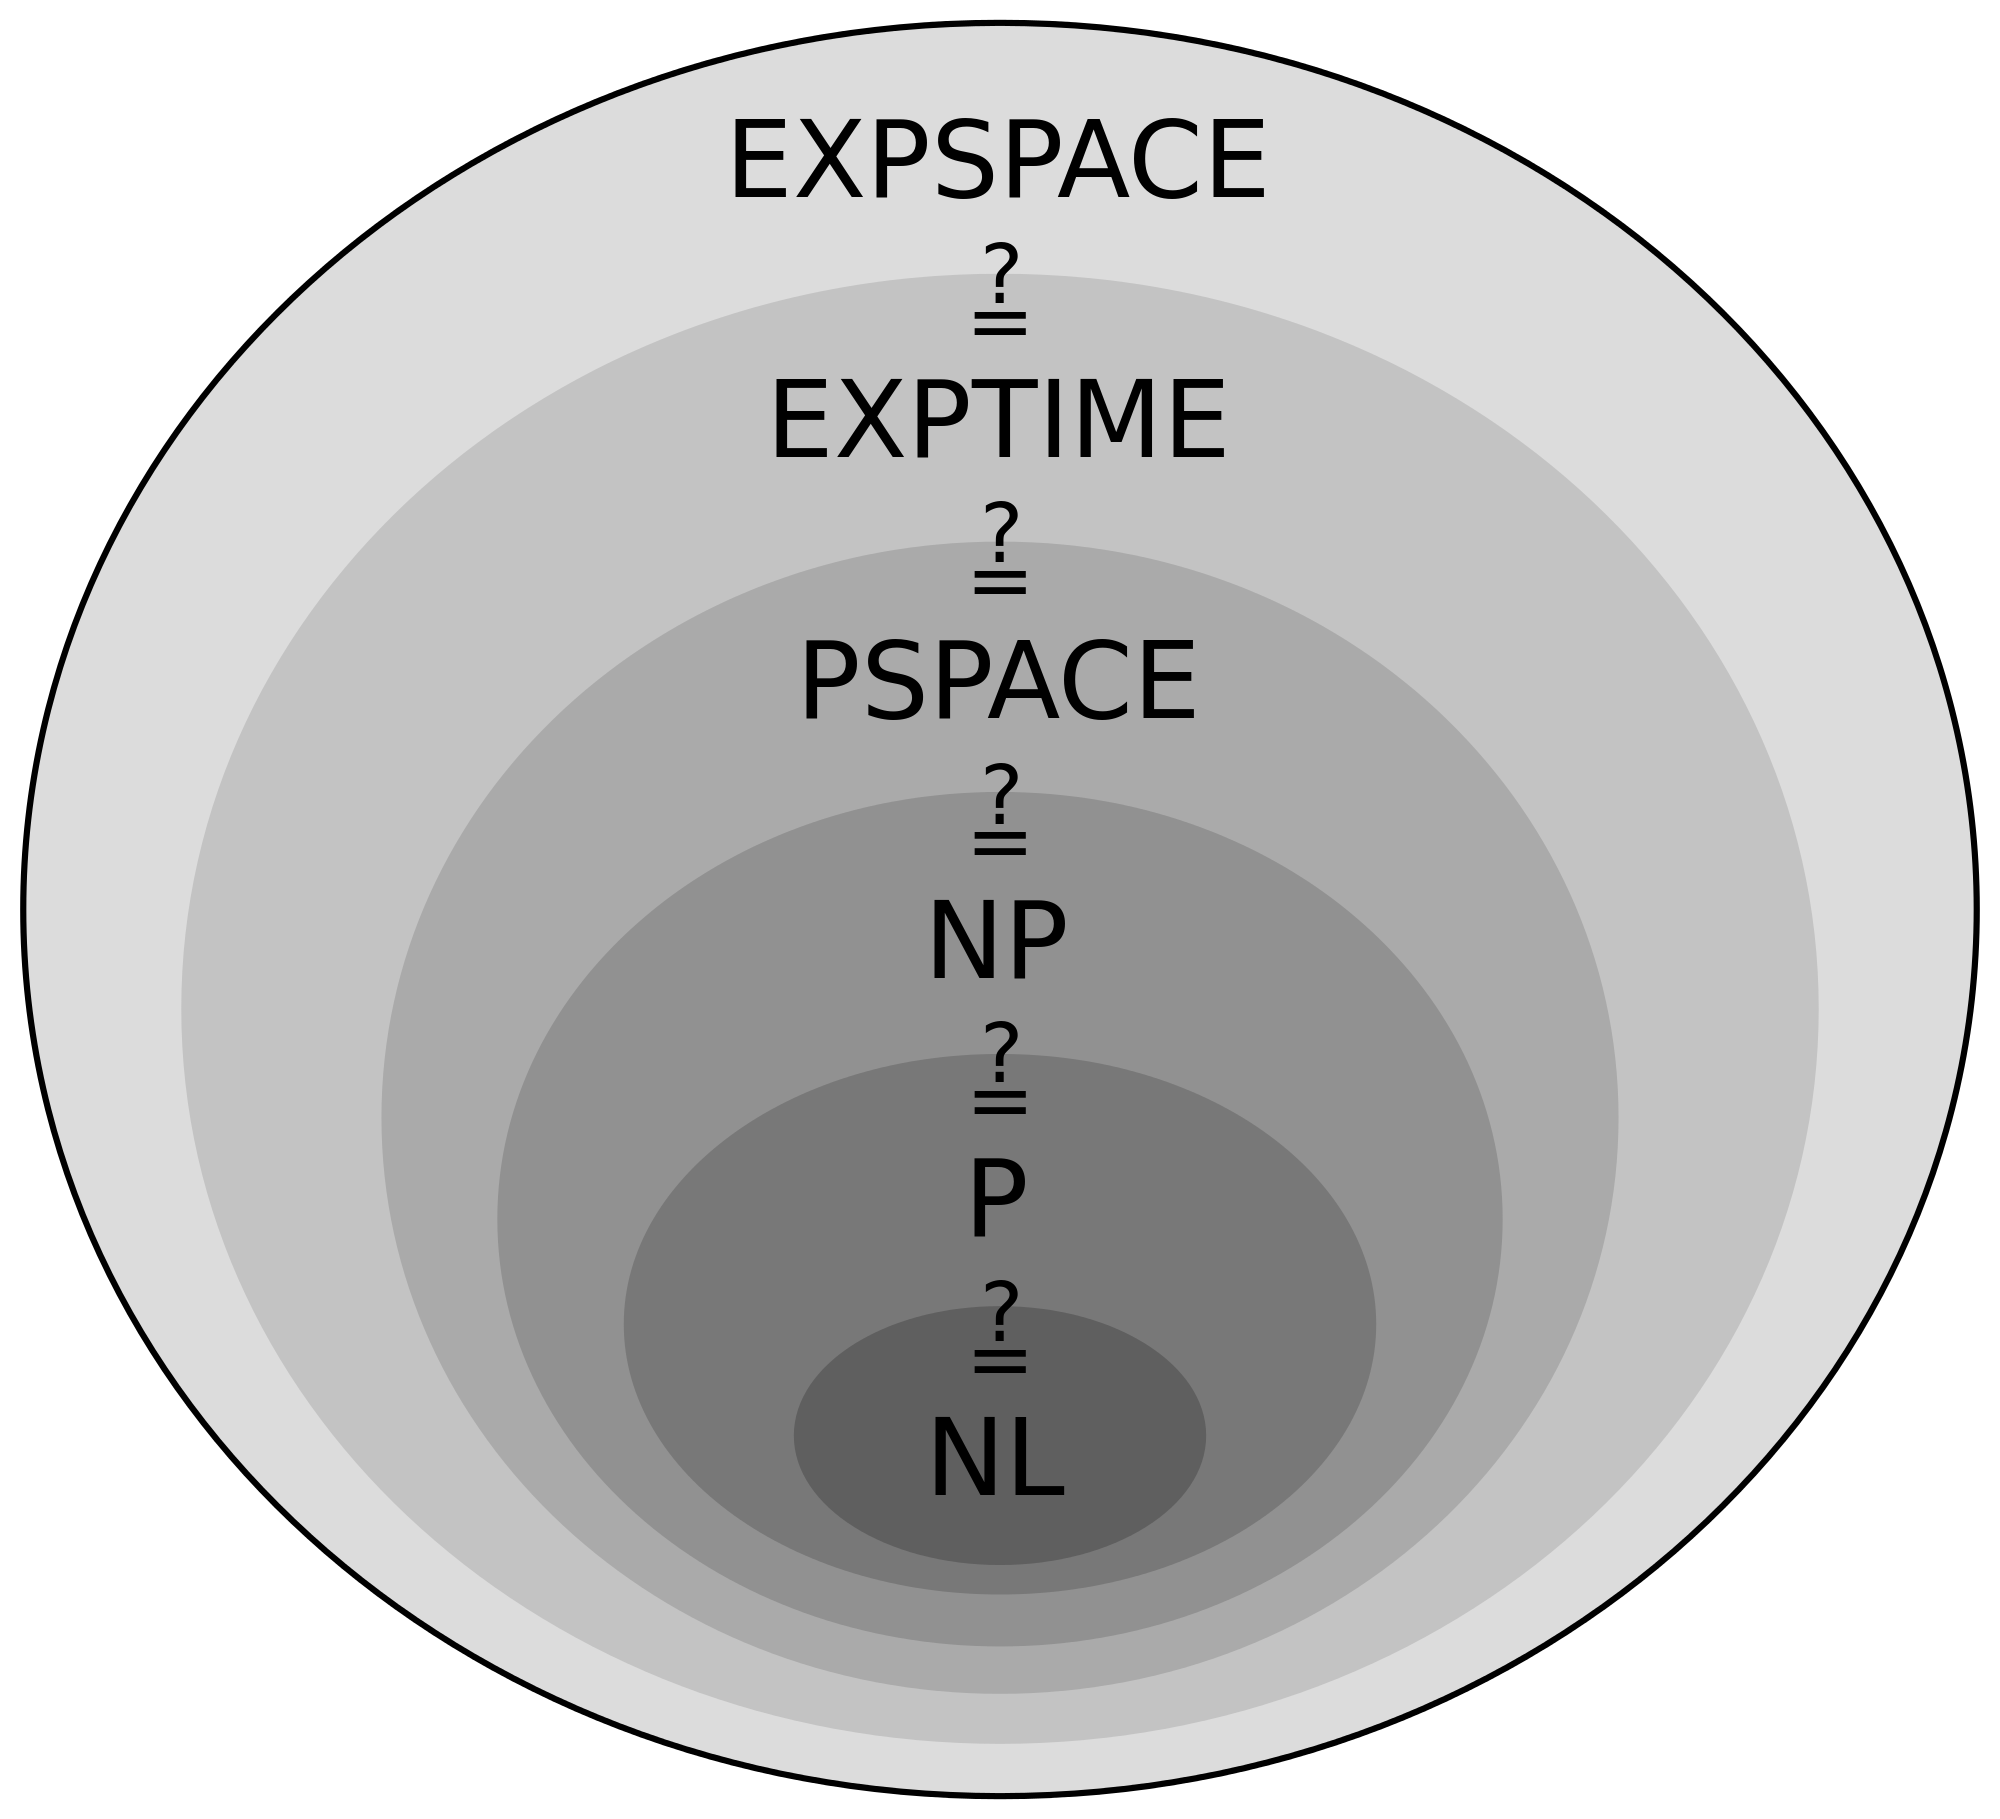
\includegraphics[width=\textwidth]{media/complexity.png}}
  \end{center}
\end{frame}

\begin{frame}{Measuring Input Size}

  Classically, we only care about input length.

  \begin{center}
    \textbf{Input 1:}
    \tape{q}{{$\cdots$, $r_1$, $r_2$, $r_3$, $r_4$, $\cdots$}}
  \end{center}

  \begin{center}
    \textbf{Input 2:}
    \tape{q}{{$\cdots$, $r_1$, $r_2$, $r_3$, $r_4$, $r_5$, $r_6$,
        $r_7$, $r_8$, $r_9$, $\cdots$}}
  \end{center}

\end{frame}

\begin{frame}{Measuring Input Size}

  Now might care abut individual entry size.

  \begin{center}
    \textbf{Input 1:}
    \tape{q}{{$\cdots$, $1$, $3$, $\pi$, $\sqrt{2}$, $\cdots$}}
  \end{center}

  \begin{center}
    \textbf{Input 2:}
    \oldheadtape[2]{q}{{$\cdots$, $2^{99}$, $3$, $\pi$, $\sqrt{2}$, $\cdots$}}
  \end{center}\pause

  Define ``magnitude'' of a cell element using a height function:
  $$\mfunctype{ht_R}{R}{\reals}.$$
\end{frame}

\begin{frame}{Measuring Input Size}
  
  For $x \in R^n$,
  \begin{itemize}
  \item[] $\len(x) = n$.
  \item[] $\size(x) = \len(x)\max_{1 \leq i \leq n}(ht_R(x_i))$.
  \end{itemize}
  
\end{frame}

\begin{frame}{Measuring Computation Cost}
  
  Let $M$ be a BSS Machine over $R$, with height function $ht_R$.
  
  \vspace{\baselineskip}

  If $\compute_M(x) = (z_0, z_1, z_2, \ldots, z_T)$, then:
  $$\cost(\compute_M(x)) = T\times ht_{max}(x).$$
  
\end{frame}

\begin{frame}{The Class $\p$}
  
  A decision problem $D$ is in class $\p$ if there exists a BSS
  Machine $M$ and constants $c, q \in \reals$ such that:
  \begin{itemize}
  \item $M$ decides $D$,
  \item For every $x \in D$, $\cost(\compute_M(x)) < c \times \size(x)^d$.
  \end{itemize}
  
\end{frame}

\begin{frame}{The Outline Strikes Back}
  \begin{center}
    \scaletopagewidth{\outlinefinal}
  \end{center}
\end{frame}

\begin{frame}{Verifiers}

  Recall our \subsum{} instance:

  \vspace{\baselineskip}

  $(\;\set{1,4,7,-5,-3,18,-6,12}\;, \;10\;)$

  \vspace{\baselineskip}

  Notice that the subset $\set{18, -3, -6, 1}$ is a short ``proof''
  that this is a Yes Instance.

  \vspace{\baselineskip}

\end{frame}

\begin{frame}{Verifiers}

  A machine $M$ taking inputs $(x, w)$ is a \textbf{verifier} for a decision
  problem $D$ if:

  \begin{itemize}
  \item[] For all $x \in D$, there exists a $w$ such that $M$ accepts
    $(x, w)$ if and only if $x \in D_{yes}$.
  \end{itemize}\pause

  A verifier for a problem $D$ is a machine that can use ``proofs'' to
  check if some input is a Yes Instance.\pause

  \vspace{\baselineskip}

  In our example: 
  \begin{align*}
    x &= (\;\set{1,4,7,-5,-3,18,-6,12}\;, \;10\;) \\
    w &= \set{18, -3, -6,1}.
  \end{align*}
\end{frame}

\begin{frame}{The Class $\np$}

  A problem $D$ is in class $\np$ if there exists a machine $M$ over
  $R$ and constants $c, q$ such that:

  \begin{itemize}
    \item M is a verifier for $D$.
    \item If $x \in D_{yes}$, then there exists a $w$ such that $M$
      accepts $(x, w)$ with $\cost(\compute_M(x, w)) \leq c \times
      size(x)^d$.
    \end{itemize}
  
\end{frame}

\begin{frame}{$\hn_R \in \np$}

  Easy to construct a verifier for $\hn_R$ with unit cost.

  \vspace{\baselineskip}

  \textbf{Algorithm:}

  Given an encoding $\set{p_1, p_2, \ldots, p_k} \subset \polyn{K}$,
  and a witness $w$, plug in first $n$ values of $w$ to each $p_i$.

  \vspace{\baselineskip}

  Accept if all $p_i$ evaluate to $0$, otherwise reject.

\end{frame}

\begin{frame}{Return of the Outline}
  \begin{center}
    \scaletopagewidth{\outlinefinal}
  \end{center}
\end{frame}

\begin{frame}{Nondeterministic Turing Machines}

  \begin{columns}

    \column{0.5\textwidth}
    Standard TM Transition:
    \functype{\delta}{(Q \times \Gamma)}{(Q \times \Gamma \times
      \set{\leftarrow, \rightarrow})}
       
    \column{0.5\textwidth}

    \begin{center}
      \detercomptm{}
    \end{center}
  \end{columns}
\end{frame}

\begin{frame}{Nondeterministic Turing Machines}

  \begin{columns}

    \column{0.5\textwidth}
    Nondeterministic TM Transition:
    \functype{\delta}{(Q \times \Gamma)}{\power{Q \times \Gamma \times
      \set{\leftarrow, \rightarrow}}}
       
    \column{0.5\textwidth}

    \begin{center}
      \scaletopagewidth{\ndetercomptm{}}
    \end{center}
  \end{columns}
\end{frame}

\begin{frame}{\ndet Machines}

  For standard BSS Machines, branch nodes defined by a pair
  $(\beta^+, \beta^-)$, plus a branching function $h$.\pause

  \vspace{\baselineskip}

  \textbf{Idea:} Let branch nodes have multiple Yes and No nodes.
  Accept $x$ if any valid sequence of configurations starting from
  $(\eta_1, I(x))$ leads to an accept state.\pause
  
  \vspace{\baselineskip}

  An \ndet Machine's branch nodes are defined by a branching function,
  plus two nonempty \textbf{sets}:

  $$\beta^+_\eta = \set{\yesnode{1}, \yesnode{2}, \ldots, \yesnode{i}}$$
  $$\beta_\eta^- = \set{\nonode{1}, \nonode{2}, \ldots, \nonode{j}}$$
\end{frame}

\begin{frame}{\ndet Computations}
  
  \begin{columns}
    
    \column{0.5\textwidth}
    \textbf{BSS Machine Computation}
    \begin{center}
      \detercompbss{}
    \end{center}
    \column{0.5\textwidth}
    \textbf{\ndet Machine Computation}
    \begin{center}
      \scaletopagewidth{\ndetercompbss{}}
    \end{center}
  \end{columns}

\end{frame}

\begin{frame}{$\ndetp$}

  A problem $D$ is in $\ndetp$ if there exists an \ndet Machine $M$
  and constants $c, q$ such that 
  \begin{itemize}
  \item $M$ decides $D$.
  \item For every $x \in D$, $\cost(\compute_M(x)) < c \times \size(x)^d$
  \end{itemize}
  
\end{frame}

\begin{frame}{Classical Nondeterminism and Verifiability}

  For Turing Machines: 
  \begin{center}
    Poly-time Verifiable $\leftrightarrow$ Nondeterministic poly-time
    Computable.
  \end{center}
\end{frame}

\begin{frame}{Classical Nondeterminisim and Verifiability}
  $\Rightarrow$ Given an NTM $M$ deciding $D$, we can construct a
  verifier $M'$ for $D$ whose witness strings for input $x$ encode the
  sequences of nondeterministic choices made by $M$ on $x$.

  \vspace{\baselineskip}
  
  If an accepting branch exists for $M$, a corresponding witness $w$
  causes $M'$ to perform an accepting computation.
\end{frame}

\begin{frame}{Nondeterminism and Verifiability}
  $\Leftarrow$ Given a verifier $M$ for $D$ with runtime bounded by $c
  \size(x)^d$, we can construct an NTM deciding $D$ by
  nondeterministically generating all possible witnesses of size less
  than $\size(x)^d$.

  \vspace{\baselineskip}

  We then (deterministically) simulate $M$ on each pair $(x, w)$.
\end{frame}

\begin{frame}{Nondeterminism and Verifiability}
  Proof of $\Rightarrow$ direction generalizes easily to BSS Verifiers
  and \ndet{} Machines.\pause

  \vspace{\baselineskip}

  Proof of $\Leftarrow$ relies on the fact that we can
  nondeterministically generate all possible witnesses in polynomial
  time. Only true if there are finitely many possibilities for each
  coordinate of a witness.
\end{frame}

\begin{frame}{$\ndetp \subseteq \np$}
  
  \begin{theorem}
    For any ring $R$ with any height function, $\ndetp \subseteq \np$
  \end{theorem}
  
  \pause
  \vspace{\baselineskip}

  \begin{theorem}
    For any finite ring $R$, $\ndetp = \np$.
  \end{theorem}
  
\end{frame}

\begin{frame}{$\ndetp$ and Binary Witnesses}

  Define $\mathbf{DNP}_R$ to be class of problems efficiently
  verifiable using witnesses containing only 0s and 1.\pause

  \vspace{\baselineskip}

  \subsum{} is a natural example.\pause
  
  \vspace{\baselineskip}

  \textbf{Instance:} $(\;\set{1,4,7,-5,-3,18,-6,12}\;, \;10\;)$

  \textbf{$\np$ Witness:}  $\set{18, -3, -6, 1}$
  
  \textbf{$\mathbf{DNP}_R$ Witness:}  $\set{1,0,0,0,1,1,1,0}$
\end{frame}

\begin{frame}{$\ndetp$ and Binary Witnesses}

  Can use constructions similar to the classical proofs to show that
  $\ndetp = \mathbf{DNP}_R$.\pause

  \vspace{\baselineskip}

  Clearly, $\mathbf{DNP}_R \subseteq \np$.  Not known in general when
  this inclusion is strict.\pause

  \vspace{\baselineskip}

  Seems likely that $\mathbf{DNP}_R \subset \np$ for uncountable
  rings.
  
\end{frame}

\begin{frame}{$\mathbf{NP}$ and Decidability}

  Can show classically that $\mathbf{NP} \subseteq \exptime$:

  \vspace{\baselineskip}

  If $D \in \mathbf{NP}$, there is a verifier $M$ running in time
  bounded by $c \times \size(x)^d$.  If $x \in D_{yes}$, $M$ accepts some
  $(x,w)$ with $\size(w) < c \times \size(x)^d$. \pause

  \vspace{\baselineskip}

  Some standard TM can enumerate all possible $w$'s and simulate $M$
  on $(x,w)$ for all of them.
\end{frame}

\begin{frame}{$\np$ and Decidability}

  This argument fails for $\np$ over infinite rings.\pause

  \vspace{\baselineskip}

  \textbf{Counterexample:} $\hn_\integers$ is equivalent to solving
  arbitrary Diophantine equations. \pause

  \vspace{\baselineskip}

  But with respect to unit cost, $\hn_\integers \in
  \nparg{\integers}$.

  \vspace{\baselineskip}

  So $\nparg{\integers}$ contains undecidable problems with respect to
  unit cost.

\end{frame}

\begin{frame}{$\ndetp$ and Decidability}

  On the other hand, since we showed that $\ndetp$ is equivalent to
  only requiring binary witnesses, the classical proof generalizes
  perfectly well for \ndet Machines, giving us:

  $$\ndetp \subseteq \exptime$$
  
\end{frame}

\begin{frame}{Separation}
  \begin{corollary}
    With respect to unit cost, $\ndetparg{\integers} \subset \nparg{\integers}$.
  \end{corollary}
\end{frame}

\begin{frame}{Known Relations and Open Problems}

  Known (as of Blum et al. '98): 
  \begin{itemize}
  \item $\p \neq \np$ for $(\integers, =)$ with unit or bit cost, and
    $(\integers, <)$ with unit cost.
  \item Also have $\p \neq \np$ for $(\rationals, <)$.
  \item Over $\reals$, $\complexes$, and $\integers_2$, $\np \subseteq
    \exptime$.\pause
  \end{itemize}
  
  \vspace{\baselineskip}

  Open Problems:
  \begin{itemize}
  \item $\p = \np?$ for $R \in \set{\reals, \complexes, \integers_2}$
    with unit cost.
  \item $\p = \ndetp?$ for any case except $\integers$ with unit cost.
  \item $\ndetp = \np?$ for any case except $\integers$ with unit cost.
  \end{itemize}\pause

  \vspace{\baselineskip}

  Conjecture:
  \begin{itemize}
    \item For any infinite ring $R$, $\p \subset \ndetp \subset \np$.
  \end{itemize}
  
\end{frame}

\begin{frame}{Future Work}
  
  \begin{itemize}
  \item Investigation of $\ndetp$ with more unusual cost measures. \pause
  \item Examining rings of nonzero characteristic. \pause
  \item Generalizing other characterizations of $\mathbf{NP}$ to BSS
    Framework. \pause
  \item[] and of course... 
  \item Settling $\mathbf{P}$ vs. $\mathbf{NP}$.
  \end{itemize}
\end{frame}

\begin{frame}

  Thanks!

\end{frame}

\end{document}


